\begin{figure}[t]
    \centering
    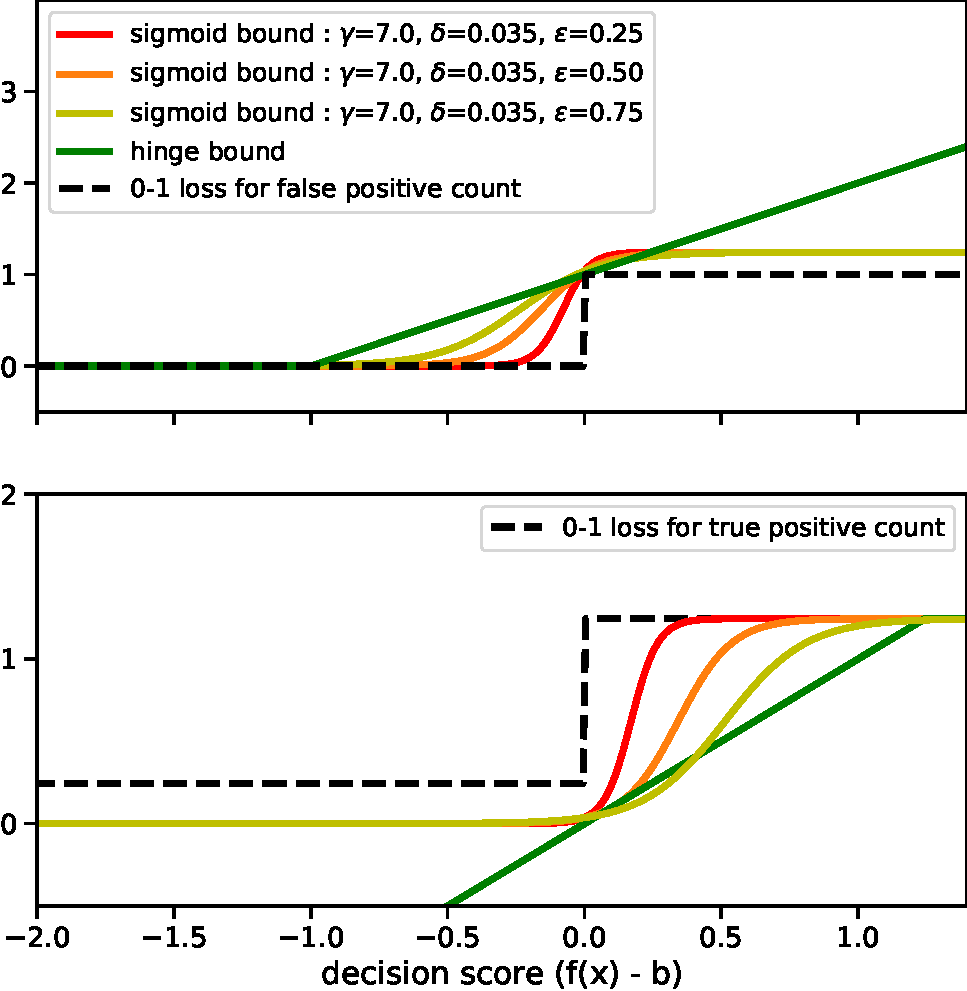
\includegraphics[height=120mm]{content/chapters/false_alarm_control/figures/tp_fp_bounds.pdf}
    \caption[Illustration of the zero-one functions and sigmoid bounds used to count false positives and true positives]{
Illustration of the zero-one functions used to count false positives (\emph{top}) and true positives (\emph{bottom}), as well as bounds that make gradient-based learning feasible.
In both plots, our family of sigmoid bounds is noticeably tighter than the hinge bound of \citet{ebanScalableLearningNonDecomposable2017}.
\emph{Bottom panel:} We bound a 0-1 loss that is \emph{vertically-shifted} by +$\gamma \delta$, so our bound is non-negative for all inputs (unlike the hinge) and thus maintains the validity of our precision constraint as discussed around Eq.~\eqref{eq:standardized_objective_constrained}.
    }%endcaption
    \label{fig:tp_fp_bounds}
\end{figure}
